\documentclass[10pt]{llncs}
\usepackage[utf8]{inputenc}
\usepackage{graphicx}
\usepackage{pgfplots}
\usepackage{amsmath} % For math mode

\definecolor{myblue}{RGB}{24,116,205}
\definecolor{myorange}{RGB}{255,127,14}
\definecolor{mygreen}{RGB}{44,160,44}

\pgfplotsset{compat=1.17} % Or your preferred version
\pgfplotsset{
legend image code/.code={
\draw [#1] (0cm,-0.1cm) rectangle (0.6cm,0.1cm);
},
}


\begin{document}
\title{Towards Secure Cross-Organizational Data Transfer: A Blockchain-Enabled Message Broker Approach}
\author{Gleb Slepenkov\orcidID{0009-0001-9978-396X}\and Vladimir Korkhov\orcidID{0000-0003-2458-3194}}
\authorrunning{G. Slepenkov}
\institute{Saint Petersburg State University, 7-9 Universitetskaya Embankment, St Petersburg, Russia, 199034\\ \email{gslepenkov@gmail.com}, \email{v.korkhov@spbu.ru}}

\maketitle

\begin{abstract}
    Secure data transmission (SDT) is crucial in modern information societies, particularly for cross-organizational data exchange. 
    This paper investigates the application of blockchain technology to create robust SDT systems, combining the benefits of using blockchain as both a data access interface and a direct data transfer tool. 
    We propose a novel architecture featuring a message broker-like design that overcomes data size limitations present in existing blockchain-based SDT solutions. 
    The architecture incorporates blockchain, internal data storage within organizations, and connectors facilitating interaction between these components. 
    The SDT process relies on smart contracts for managing data access, transfer, and confirmation, while the actual data is stored off-chain. 
    We advocate for a private, two-layered blockchain-based system, employing PBFT consensus within smaller clusters for efficient message transfer and RAFT consensus for system management and data replication. 
    This layered approach enhances both fault tolerance and scalability, paving the way for a practical and secure cross-organizational SDT system.
    We present an architectural overview and describe key implementation details of proposed system.
    
    \keywords{Blockchain \and Secure Data Transfer (SDT) \and Data Security \and Distributed Ledger Technology (DLT) \and Message Broker \and Data Access Control \and Cross-Organizational Data Sharing \and Scalability \and Fault Tolerance}
\end{abstract}

\section{Introduction}

In contemporary information societies, secure data transmission (SDT) is essential for maintaining data confidentiality and integrity.
SDT systems are critical infrastructure components across diverse sectors, including financial institutions, governmental agencies, and enterprises.

Implementing robust SDT mechanisms becomes particularly challenging when facilitating cross-organizational data exchange or connecting geographically dispersed departments within a single organization.
Such scenarios necessitate data transfer across external, public networks, thereby significantly elevating the risk of unauthorized data disclosure or modification during transit.
Consequently, rigorous data integrity verification and sender authentication protocols are indispensable.
Furthermore, confirmation of data reception is often a critical requirement.
The heterogeneity of data exchange technologies employed by different entities can further complicate the SDT process.

Blockchain represents an emerging technology for SDT solutions.
This technology by design provides core features essential for SDT, such as fault tolerance, ledger data immutability and zero trust between blockchain nodes.
Moreover, many blockchains are designed to operate in unreliable public networks with nodes running in different heterogeneous clusters owned by separate stakeholders.
For this reason, blockchains are especially suitable for cross-organizational data transfer.
Furthermore, blockchain platforms often provide smart contracts, which allow implementing custom data transfer logic directly on the blockchain.

This suitability has stimulated significant research interest, as evidenced by comprehensive surveys exploring blockchain applications for data sharing and exchange \cite{Song2023} and for specific domains like smart transport \cite{Bagga2022}.
These surveys highlight the potential of blockchain to address the challenges of SDT in diverse and demanding environments.

This study explores existing blockchain application paradigms for the SDT process and proposes a novel approach that integrates their advantages. 
The result is a blockchain-based SDT system that maintains key features of established approaches while adopting a message broker-like architecture with relaxed data size limitations. 
This article presents an architectural overview and describes key implementation details of the proposed system.

The study is organized in the following way.
Section \ref{related_work} describes existing data transfer paradigms in detail.
Section \ref{architecture} represents the proposed system architecture.
Section \ref{implementation_details} describes implementation details of the proposed system.
Finally, Section \ref{summary} concludes this article and denotes further research directions.

\section{Related Work} \label{related_work}

The integration of blockchain technology into data transfer systems presents two primary paradigms: blockchain as a data access interface and blockchain as a direct data transfer tool.
This section examines the existing literature, classifying studies according to these two distinct roles of blockchain in facilitating data exchange.

\subsection{Blockchain as a Data Access Interface}

This approach leverages blockchain as a secure and transparent mechanism for managing and controlling access to data that is typically stored off-chain.
The blockchain records metadata about the data, access permissions, and transaction histories, thereby ensuring data integrity, auditability, and secure access control.
The data itself is transferred using conventional methods.

Wang et al. introduced BBS, a big data sharing system utilizing blockchain for access control and data integrity management \cite{Wang2024}.
Similarly, Wang et al. proposed a blockchain-based model for sharing big data in the oil and gas sector, employing blockchain to enable secure data access and provenance tracking \cite{WangYY2021}.
Yang et al. developed a sharing platform for wild bird data based on blockchain and IPFS, where blockchain governs access rights to data residing in IPFS \cite{Yang2022}.
A cross-organizational data sharing framework that uses blockchain probes to orchestrate and audit data access across various entities was presented by Jia et al. \cite{Jia2023}.
Gupta et al. explored the application of blockchain for securing data access within e-healthcare applications \cite{Gupta2022}.
\subsection{Blockchain as a Data Transfer Tool}

This approach employs the blockchain directly to transfer data between participants.
While data may occasionally be stored on-chain, it is more common for the blockchain to facilitate the transfer of data stored off-chain,
 often in conjunction with technologies such as peer-to-peer networks or distributed file systems.

Lin et al. proposed a multi-level blockchain architecture for secure data transfer in the Internet of Vehicles (IoV), 
directly leveraging blockchain for data exchange \cite{Lin2023}. 
Peng et al. demonstrated the feasibility of building a peer-to-peer file storage and sharing system on a consortium blockchain, 
where the blockchain assists in discovering and securely transferring file chunks \cite{Peng2023}. 
Priyadarshini et al. introduced a system for secured data transfer between fog nodes utilizing blockchain to enhance the security of 
the data transfer process itself \cite{Priyadarshini2021}.

\subsection{Enabling Technologies and Security Considerations}

Regardless of the chosen paradigm, several enabling technologies and security considerations are universally relevant. 
Kim et al. presented a hybrid decentralized PBFT blockchain framework for OpenStack message queues, aimed at improving fault tolerance and scalability, 
crucial aspects for reliable data transfer systems \cite{kim2020hybrid}. 
A publish-subscribe architecture to foster interoperability among different blockchain networks, thus facilitating data exchange across heterogeneous systems, was introduced by Ghaemi et al. \cite{Ghaemi2021}. 
Both solutions represent the architecture where blockchain acts as a message broker, data transfer process is organized in publish-subscribe way and data flow is separated into topics. 
Such an architecture is traditional for message brokers like Apache Kafka \cite{apachekafka}.
That's why it will be referenced as "message broker-like" architecture in the rest of the paper.

Bagga et al. and Xu et al. explored blockchain-based authentication and key agreement protocols for IoV, enhancing the security of data transfer in vehicular contexts \cite{Bagga2021,Xu2021}. 
Bogdanov et al. focused on the consensus mechanism, exploring a combination of PBFT and Raft \cite{Bogdanov2024}, while Ai et al. proposed a Proof-of-Transactions consensus protocol \cite{Ai2022}, 
both striving for efficient and scalable agreement in distributed ledgers. 

\subsection{Comparison of Approaches}

The two approaches, blockchain as a data access interface and blockchain as a data transfer tool, offer distinct advantages and disadvantages depending on the specific use case and requirements.

\begin{table}[h!]
\caption{Comparison of Blockchain Approaches for Data Transfer}
\label{tab:comparison}
\begin{tabular}{|p{2.0cm}|p{5.0cm}|p{5.0cm}|}
\hline
Feature & Blockchain as Data Access Interface & Blockchain as Data Transfer Tool \\ \hline
Data Storage & Primarily Off-Chain & Often Off-Chain, but metadata on-chain \\ \hline
Data Transfer & Traditional methods & Blockchain or Blockchain-assisted \\ \hline
Scalability & Higher, as data transfer is off-chain & Potentially Lower, dependent on blockchain throughput \\ \hline
Complexity & Lower & Higher \\ \hline
On-Chain Footprint & Smaller (Metadata only) & Larger (Metadata and potentially data chunks) \\ \hline
Suitability & Large datasets, access control focus & Smaller datasets, secure and direct transfer focus \\ \hline
\end{tabular}

\end{table}

As illustrated in Table \ref{tab:comparison}, the choice between these two approaches hinges on factors such as data size, scalability requirements, security priorities, 
and the level of on-chain transparency desired. 
The data access interface approach is generally more suitable for scenarios involving large datasets and a primary focus on secure access control, while the data transfer tool 
approach is better suited for scenarios demanding secure and direct data transfer, even if it potentially introduces limitations in terms of scalability.

\section{System Architecture Overview} \label{architecture}

\subsection{System Components}

This section describes the architecture of the proposed system. 
The architecture aims to combine two dominant blockchain integration paradigms for data transfer systems, as identified in Section \ref{related_work}. 
By integrating these approaches, our system seeks to achieve a message broker-like architecture that facilitates convenient data transfer while mitigating the data size limitations inherent in individual solutions.

Our architecture leverages the following trends observed in recent research:

\begin{enumerate}
    \item \textbf{Blockchain as a message broker:} (e.g., \cite{Ghaemi2021}, \cite{kim2020hybrid}). This approach utilizes the blockchain ledger for direct message transfer.
    \item \textbf{Blockchain as an interface to off-chain data:} (e.g., \cite{Jia2023}, \cite{Wang2024}). This paradigm employs the blockchain to manage access and pointers to data stored off-chain.
\end{enumerate}

While each of these trends offers unique advantages, they also present limitations:

\begin{enumerate}
    \item \textbf{Limitations of Blockchain as a Message Broker:} Relying on the blockchain ledger for message transfer significantly restricts system scalability and the size of transmissible data due to the inherent constraints of blockchain technology.

    \item \textbf{Limitations of Blockchain as an Interface to Off-Chain Data:} Solutions implementing this approach often lack native notification mechanisms, making efficient message retrieval a challenge and requiring external polling or other complex notification strategies.
\end{enumerate}

The proposed system addresses these individual limitations by combining the strengths of both paradigms. 
This integrated approach allows us to leverage the blockchain for both message brokering and off-chain data referencing, effectively relaxing the constraints on data size and enabling efficient notification mechanisms. 

The proposed architecture assumes that the system should contain the following components:

\begin{itemize}
    \item Blockchain as the core system component responsible for data transfer process orchestration. 
    Blockchain nodes act as interfaces to data storages, while smart contracts implement all data transfer mechanisms like
    data transformation (e.g. message encryption / signing), data verification and message notifications. 
    \item Data storages internally used by counterparties (organizations) to store the data to be sent.
    \item Connectors --- some application used by SDT process counterparties in order to create a connection between their data storages
    and blockchain nodes owned by the organization (mainly inspired by blockchain probes described in \cite{Jia2023}).
\end{itemize}

A sample of such an architecture for SDT between two organizations is presented in Figure \ref{system_architecture}.

\begin{figure}[ht!]
    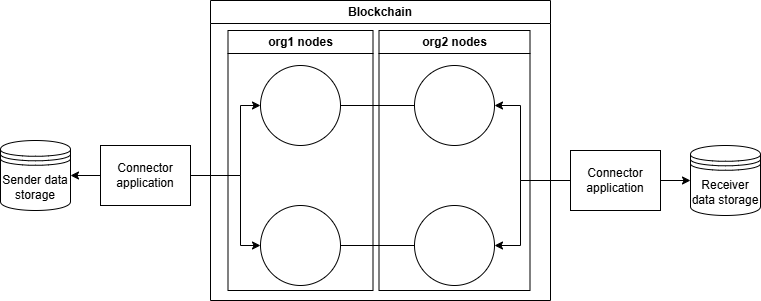
\includegraphics[width=\textwidth]{system_architecture.png}
    \caption{System architecture for two organizations} \label{system_architecture}
\end{figure}

\subsection{SDT Process Scheme}

The SDT process scheme is illustrated in Figure \ref{sending_process} and involves data transfer between two organizations (Org1 and Org2) using a blockchain-mediated system. 

\begin{figure}[ht!]
    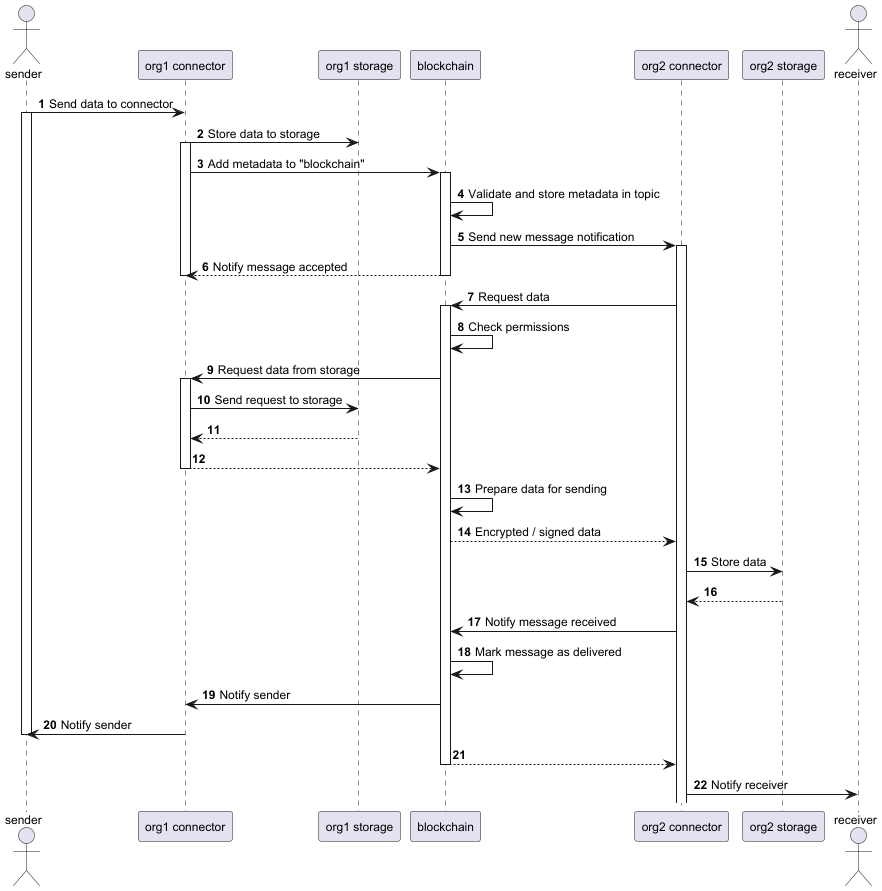
\includegraphics[width=\textwidth]{sending_process.png}
    \caption{SDT process scheme} \label{sending_process}
\end{figure}

The process can be separated into following stages:

\subsubsection{Data Sending (Org1)}

\begin{enumerate}
    \item \textbf{Initiate Transfer (1):} The data sender (Org1) initiates a data transfer request to its connector.
    \item \textbf{Data Persistence and Metadata Collection (2):} The Org1 connector persists the data in Org1's storage and gathers associated metadata.
    \item \textbf{Smart Contract Invocation (3):} The Org1 connector queries the blockchain to initiate the execution of the SDT smart contract.
    \item \textbf{Metadata Validation and Recording (4):} The smart contract validates the provided metadata and records it on the ledger.
    \item \textbf{Notification (5-6):} Upon successful metadata validation, the smart contract notifies the Org2 connector about the availability of a new message and acknowledges message acceptance to Org1.
\end{enumerate}

\subsubsection{Data Retrieval (Org2)}

\begin{enumerate}
    \item \textbf{Data Request and Smart Contract Execution (7):} The Org2 connector queries the blockchain nodes and executes the SDT smart contract.
    \item \textbf{Receiver Authentication (8):} The smart contract verifies Org2's permissions to the requested data.
    \item \textbf{Data Retrieval from Org1 (9-12):} If authorized, the smart contract requests the data from the Org1 connector.  
    Upon receiving the request, the Org1 connector retrieves the data from Org1's storage and transmits it back to the smart contract.
    \item \textbf{Data Preparation (13):} The smart contract prepares the data for transfer, potentially involving encryption and digital signing.
    \item \textbf{Data Delivery to Org2 (14-16):} The prepared data is returned to the Org2 connector, which then stores the received data in Org2's storage.
\end{enumerate}

\subsubsection{Process Finalization}

\begin{enumerate}
    \item \textbf{Message Reception Notification (17):} The Org2 connector notifies the blockchain about the message reception via the smart contract.
    \item \textbf{Message Registry Update (18):} The smart contract updates the message registry, marking the message as delivered.
    \item \textbf{Confirmation Notifications (19-22):} The smart contract notifies the Org1 and Org2 connectors about the successful completion of the message delivery process, 
    and the connectors inform the data sender and data receiver about the completion of the data transfer process respectively.
\end{enumerate}

Such an algorithm has the following important features:

\begin{enumerate}
    \item Loose coupling between sender and receiver due to blockchain usage as a message broker.
    \item Better fault tolerance compared to regular message brokers.
    \item More convenient message broker-like SDT interface compared to existing blockchain solutions.
    \item Greater SDT process customization capabilities due to smart contract usage.
\end{enumerate}

\section{Implementation details} \label{implementation_details}

\subsection{Blockchain Selection}

Blockchain technology constitutes the core component of the SDT system. 
Consequently, the specific blockchain implementation exerts a significant influence on key system parameters, including:

\begin{itemize}
    \item \textbf{Throughput:} The volume of data the system can transfer within a defined time interval.
    \item \textbf{Fault Tolerance:} The types of faults the system can withstand and the maximum number of node failures the system can accommodate while maintaining functionality.
    \item \textbf{Scalability:} The maximum permissible number of nodes within the system.
\end{itemize}

The parameters delineated above are primarily governed by the blockchain type and the employed consensus algorithm.

A review of the existing literature reveals a prevalent trend favoring private blockchain solutions. 
This preference arises from the necessity for controlled access, enhanced privacy, and the potential for higher throughput in many SDT scenarios, particularly within applications such as IoT and vehicular networks. 
While several studies mention the potential use of public blockchains, they are not typically presented as the primary option.  
Specific examples include:

\begin{itemize}
    \item Peng et al. \cite{Peng2023} propose a peer-to-peer file storage and sharing system based on a consortium blockchain.
    \item Jia et al. \cite{Jia2023} present a cross-organizational data sharing framework based on blockchain-probes, indicative of a permissioned setting.
    \item Numerous papers addressing IoT applications (e.g., \cite{Ai2022,Gupta2022}) often implicitly or explicitly assume a permissioned blockchain context to address security and scalability constraints.
\end{itemize}

Therefore, this paper posits that a private blockchain is the most suitable option for SDT system implementation.

In addition to selecting the appropriate blockchain type, employing the correct consensus algorithm is crucial. 
To enhance the SDT system's fault tolerance, this paper proposes the utilization of the Practical Byzantine Fault Tolerance (PBFT) algorithm, aligning with observed trends in the literature. 
However, PBFT is known to have inherent performance limitations.

Firstly, PBFT implementations necessitate the transfer of substantial data volumes between blockchain nodes to achieve consensus. 
For instance, the BFT-SMaRT algorithm, employed by Hyperledger Fabric \cite{barger2021byzantine}, requires each node to transmit 80 MB of data to achieve a performance of 2500 transactions per second. 
This implies a total traffic volume of 720 MB within a cluster of only 10 nodes during all consensus algorithm stages.

Furthermore, the throughput of such a consensus algorithm is contingent upon the number of nodes within the system. 
Research \cite{barger2021byzantine} indicates that BFT-SMaRT achieves maximum throughput when the system comprises 7 nodes (Fig. \ref{fig:smartbft-global}).

\begin{figure}
    \centering
    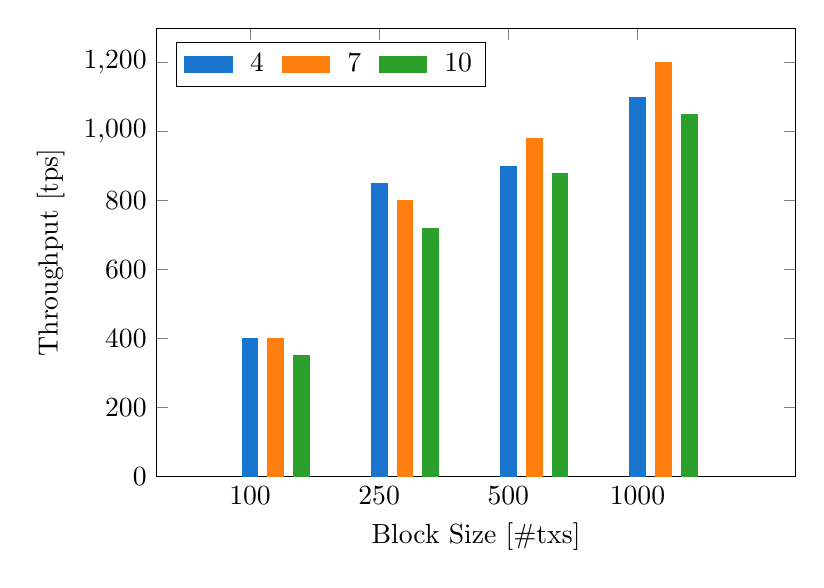
\begin{tikzpicture}
        \begin{axis}[
            width=0.8\textwidth, 
            height=0.6\textwidth,
            xlabel={Block Size [\#txs]},
            ylabel={Throughput [tps]},
            xmin=0, xmax=4.5,
            ymin=0, ymax=1300,
            xtick={0.5,1.5,2.5,3.5},
            xticklabels={100,250,500,1000},
            legend pos=north west,
            ymajorgrids=false,
            bar width=0.2cm,
            enlarge x limits=0.05,
            legend style={
                legend columns=3, 
                column sep=1ex,  
                row sep=0.2ex  
             },
         ]
        % Data for Cluster Size 4
        \addplot[ybar, solid, draw=myblue, color=myblue, fill=myblue] coordinates {
            (0.5, 400)
            (1.5, 850)
            (2.5, 900)
            (3.5, 1100)
        };
        \addlegendentry[solid]{4}

        % Data for Cluster Size 7
        \addplot[ybar,color=myorange, fill=myorange] coordinates {
            (0.7, 400)
            (1.7, 800)
            (2.7, 980)
            (3.7, 1200)
        };
        \addlegendentry{7}

        % Data for Cluster Size 10
        \addplot[ybar,color = mygreen, fill=mygreen] coordinates {
            (0.9, 350)
            (1.9, 720)
            (2.9, 880)
            (3.9, 1050)
        };
        \addlegendentry{10}

        \node at (axis cs:0.7,3700) [anchor=south west]{Cluster Size};
    \end{axis}
    \end{tikzpicture}
    \caption{BFT-SMaRT performance in global networks (measured by Barger et. al. \cite{barger2021byzantine})}
    \label{fig:smartbft-global}
\end{figure}

Increasing the number of nodes beyond this optimum leads to a degradation in throughput. 
The maximum permissible number of nodes, according to research \cite{Ke2023}, is limited to approximately 100.

For the reasons articulated above, a pure PBFT blockchain is not ideally suited for the creation of scalable and fault-tolerant systems. 
Fortunately, this limitation can be addressed by leveraging the multi-layered blockchain architecture described in \cite{Bogdanov2024} and \cite{Lin2023}, 
coupled with the data flow separation into topics and partitions, a common practice in message brokers such as Apache Kafka \cite{apachekafka}.

This paper proposes the use of a two-layered blockchain architecture. 
The first layer employs the PBFT consensus algorithm.  
Given the algorithm's known limitations, this layer will be constructed from multiple, relatively small clusters, each consisting of up to 7 nodes. 
This layer embodies the concept of a partition, representing the smallest system component directly responsible for the execution of SDT smart contracts.

The subsequent layer leverages the RAFT consensus algorithm \cite{ongaro2015raft}. 
This layer is designed for two primary functions: system management (detailed in Section \ref{data-flow}) and asynchronous data replication following PBFT consensus rounds (described in Section \ref{data-replication}). 
Consequently, this layer is analogous to the topic concept found in message brokers.

This architecture allows for the preservation of all fault-tolerance characteristics inherent in the PBFT consensus algorithm while simultaneously enhancing system scalability. 
Scaling the system does not necessitate an increase in the PBFT cluster size. 
Instead, a new, smaller PBFT layer-1 cluster is created and connected to the existing RAFT layer-2 cluster, which has a less stringent limit on the maximum number of nodes.

\subsection{Data Flow Separation}\label{data-flow}

This section delineates the proposed data flow separation scheme. 
As previously mentioned, the data flow of the SDT system is partitioned into topics and partitions.

A topic is defined as a data stream unified by a common theme or a list of consumers. 
To address the limitations outlined earlier, each topic is further subdivided into a list of partitions.
 An illustrative example of such a data flow separation into two partitions is depicted in Fig. \ref{blockchain_layers}.

\begin{figure}
    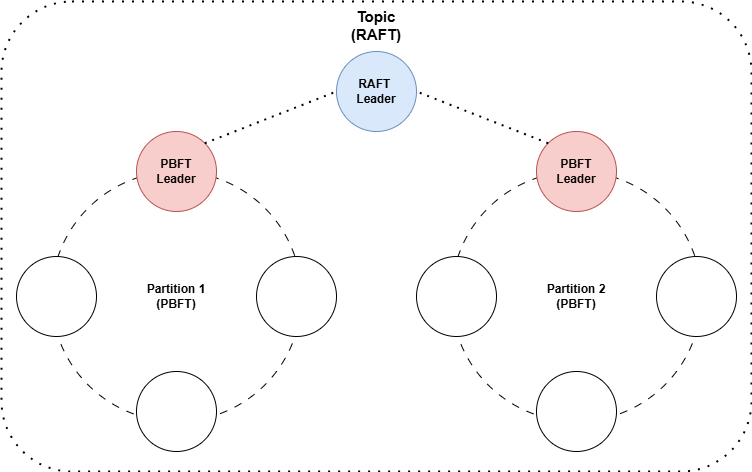
\includegraphics[width=\textwidth]{two-layered-blockchain.png}
    \caption{Structure of a topic with two partitions} \label{blockchain_layers}
\end{figure}

Two primary challenges must be addressed to implement this data flow separation:

\begin{itemize}
    \item How to select a specific blockchain node for SDT process initialization while ensuring effective load balancing?
    \item How to select the appropriate partition for a specific message?
\end{itemize}

The selection of a specific load balancing algorithm constitutes a separate area of research and, therefore, falls outside the scope of this article.

Concerning the second challenge, this paper proposes the utilization of hash partitioning, a technique employed by Apache Kafka, for partition selection.  
The partition is determined by calculating the remainder of dividing the key's hash value by the total number of partitions.

To store the topic configuration data, the layer-2 ledger of the blockchain is proposed. 
Each node within this blockchain layer stores a list of partitions and a corresponding list of nodes for each partition. 
Any structural modifications within a topic, such as the creation of a new partition, are to be executed via a dedicated smart contract.

A key advantage of this approach lies in the replication of configuration data across all blockchain nodes. 
Consequently, data senders can retrieve this data from any topic node. 
This eliminates the need for dedicated control nodes, such as Apache Zookeeper nodes in Apache Kafka, thereby enhancing system fault tolerance by mitigating the risk of a single point of failure.


\subsection{Data Replication}\label{data-replication}
As previously discussed, a primary advantage of utilizing blockchain technology in a data transfer system is its ability to provide verifiable evidence of message delivery by immutably recording the data transfer history within its ledger.
 Given the system's separation into multiple partitions, verifying message delivery necessitates identifying the specific partition used for the message's transmission. 
 This task is complicated by the fact that the system configuration may evolve over time, potentially requiring an iterative search across all existing partitions.
 To streamline the message delivery verification process, data replication to all topic nodes is essential.

To facilitate this data replication mechanism, this article introduces the concepts of global and local ledgers. 
The global ledger, maintained at the topic level, essentially represents the union of all partition-specific ledgers, which we term local ledgers. 
The global ledger is updated asynchronously with data from the local ledgers through a dedicated periodic task. 
This task implements the following algorithm:

\begin{enumerate}
    \item Retrieve the list of partitions from the topic configuration ledger.
    \item For each partition:
    \begin{enumerate}
        \item Identify the key of the last replicated block.
        \item Query the local partition ledger to ascertain the presence of new data.
        \item If new data is found, copy all new data blocks to the global ledger.
    \end{enumerate}
\end{enumerate}

An illustrative example of this algorithm's execution for two partitions is presented in Fig. \ref{global-and-local-ledgers}. 
In the figure, the last replicated blocks are highlighted in yellow, while the blocks slated for replication are depicted in green. 
Prior to the algorithm's execution, there are three blockchain nodes awaiting replication: one from Partition 1 and two from Partition 2. 
Following the replication process, these blocks are appended to their corresponding blockchains within the global ledger.

\begin{figure}[ht!]
    \centering
    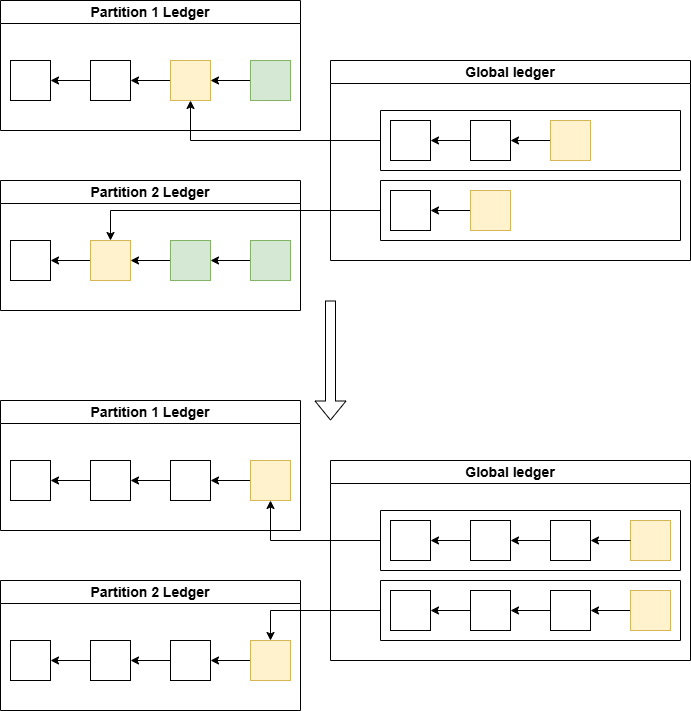
\includegraphics[width=0.7\textwidth]{global-and-local-ledgers.png}
    \caption{Data replication to global ledger} \label{global-and-local-ledgers}
\end{figure}

Given that the algorithm operates on the second blockchain layer, all modifications to the global ledger are, again, governed by the RAFT consensus algorithm.


\section{Supposed AI Application Approaches}

The integration of Artificial Intelligence (AI) with blockchain technology offers promising avenues for enhancing the performance, security, and efficiency of smart contract execution.  
Specifically, AI can be leveraged in two crucial areas: anomaly detection within smart contracts and dynamic load balancing of smart contract execution requests.

\subsection{Anomaly Detection in Smart Contracts}

Smart contracts, while offering automated execution of agreements, are susceptible to vulnerabilities that can lead to significant financial losses.  
Employing AI, particularly deep learning techniques, enables the development of sophisticated anomaly detection systems capable of identifying malicious code or unexpected behavior within smart contracts. 
As highlighted in \cite{Demertzis2020}, blockchain-enabled deep learning can be utilized to create smart contracts that autonomously detect anomalies, thereby improving the security and reliability of Industry 4.0 applications.  
In case of the SDT systems, AI could be used to detect anomalies in SDT process, such as data corruption or unexpected workload changes.

\subsection{AI-Driven Load Balancing for Smart Contract Execution}

As the demand for smart contract execution increases, optimizing the allocation of computational resources across the blockchain network becomes crucial. 
AI algorithms can be employed to dynamically balance the load of smart contract execution requests across different nodes in the network.
 This approach allows for smart selection of the most appropriate node based on various parameters, such as node availability, computational capacity, network latency, and current workload.  
 Singh et al. \cite{Singh2024} demonstrate the potential of AI-integrated blockchain frameworks for optimizing load balancing, particularly in the context of smart EV charging networks. 
 By leveraging AI, the system can predict the demand for charging and intelligently distribute the workload across available charging stations, which is analogous to smart contract execution across different nodes.  
 This dynamic load balancing leads to improved network throughput, reduced latency, and enhanced overall system efficiency. 
 This concept can also be transferred to other applications using blockchain and AI, as shown by Tsang et al. \cite{Tsang2024}.
 In case ot system proposed in this article, AI could be especially useful for load balancing at the partition level in order to select the specific node to start smart contract execution process.

\section{Summary} \label{summary}

This paper introduces a novel and secure architecture for cross-organizational data transfer (SDT) that leverages the strengths of blockchain technology. 
Addressing the limitations of existing blockchain-based SDT solutions, which often struggle with data size constraints and notification mechanisms, our approach combines the "blockchain as a data access interface" and "blockchain as a direct data transfer tool" paradigms. 
This innovative architecture adopts a message broker-like design, enabling efficient data exchange while mitigating the inherent restrictions on data size. 
The proposed system comprises a blockchain core, internal organizational data storages, and connectors that seamlessly link these storage facilities to blockchain nodes. 
The SDT process is orchestrated via smart contracts, which handle data access control, transfer management, and confirmation procedures, with the actual data residing off-chain within the organization's secure storage. 
To optimize performance and security, we propose a private, two-layered blockchain structure. 
The first layer utilizes PBFT consensus within smaller clusters, facilitating rapid message transfer within partitions, while the second layer employs RAFT consensus for robust system management and asynchronous data replication across topics.
This layered design significantly enhances fault tolerance and scalability, offering a substantial improvement over single-layer blockchain implementations. 
By providing a loose coupling between sender and receiver, improved fault tolerance compared to traditional message brokers, a more convenient message broker-like SDT interface, and greater SDT process customization capabilities through smart contract usage, 
this architecture presents a practical and secure solution for cross-organizational data sharing.

Future research will focus on several key areas to further refine and validate the proposed architecture. 
These include the implementation and evaluation of a functional prototype to assess real-world performance, the selection of specific, optimized consensus algorithm implementations, 
and the development of a dynamic load balancing mechanism for intelligent partition selection to ensure optimal resource utilization and system responsiveness.

\bibliographystyle{splncs04}
\bibliography{references}

\end{document}